\documentclass[CJK]{beamer}
\usepackage{CJKutf8}
\usepackage{beamerthemesplit}
\usetheme{Malmoe}
\useoutertheme[footline=authortitle]{miniframes}
\usepackage{amsmath}
\usepackage{amssymb}
\usepackage{graphicx}
\usepackage{color}
\usepackage{slashed}
\usepackage{simplewick}
\graphicspath{{../figures/}}
\def\be{\begin{equation}}
\def\ee{\nonumber\end{equation}}
\def\bea{\begin{eqnarray}}
\def\eea{\nonumber\end{eqnarray}}
\def\ii{{\dot{\imath}}}
\def\bch{\begin{CJK}{UTF8}{gbsn}}
\def\ech{\end{CJK}}
\def\bex{\begin{minipage}{0.3\textwidth}
\includegraphics[width=1in]{jugelizi.png}\end{minipage}\begin{minipage}{0.6\textwidth}}
\def\eex{\end{minipage}}
\def\chtitle#1{\frametitle{\bch#1\ech}}
\def\skipline{{\vskip0.1in}}
\def\skiplines{{\vskip0.2in}}
\def\lagr{{\mathcal{L}}}
\def\hamil{{\mathcal{H}}}
\def\vecv{{\mathbf{v}}}
\def\vecx{{\mathbf{x}}}
\def\veck{{\mathbf{k}}}
\def\vecp{{\mathbf{p}}}
\def\vecn{{\mathbf{n}}}
\def\vecA{{\mathbf{A}}}
\def\vecP{{\mathbf{P}}}
\def\vecsigma{{\mathbf{\sigma}}}
\def\hatJn{{\hat{J_\vecn}}}
\def\hatJx{{\hat{J_x}}}
\def\hatJy{{\hat{J_y}}}
\def\hatJz{{\hat{J_z}}}
\def\hatj#1{\hat{J_{#1}}}
\def\hatphi{{\hat{\phi}}}
\def\hatq{{\hat{q}}}
\def\hatpi{{\hat{\pi}}}
\def\vel{\upsilon}
\def\Dint{{\mathcal{D}}}
\def\adag{{\hat{a}^\dagger}}
\def\bdag{{\hat{b}^\dagger}}
\def\cdag{{\hat{c}^\dagger}}
\def\ddag{{\hat{d}^\dagger}}
\def\hata{{\hat{a}}}
\def\hatb{{\hat{b}}}
\def\hatc{{\hat{c}}}
\def\hatd{{\hat{d}}}
\def\hatN{{\hat{N}}}
\def\hatH{{\hat{H}}}
\def\hatp{{\hat{p}}}
\def\Fup{{F^{\mu\nu}}}
\def\Fdown{{F_{\mu\nu}}}
\def\newl{\nonumber \\}
\def\SIkm{\mathrm{km}}
\def\SIyr{\mathrm{yr}}
\def\SIGyr{\mathrm{Gyr}}
\def\SIeV{\mathrm{eV}}
\def\SIGeV{\mathrm{GeV}}
\def\SIm{\mathrm{m}}
\def\SIcm{\mathrm{cm}}
\def\SIJ{\mathrm{J}}
\def\SIs{\mathrm{s}}
\def\SIkg{\mathrm{kg}}
\def\SIg{\mathrm{g}}
\def\vece{\mathrm{e}}
\def\bmat#1{\left(\begin{array}{#1}}
\def\emat{\end{array}\right)}
\def\bcase#1{\left\{\begin{array}{#1}}
\def\ecase{\end{array}\right.}
\def\calM{{\mathcal{M}}}
\def\calT{{\mathcal{T}}}
\def\calR{{\mathcal{R}}}
\def\barpsi{\bar{\psi}}
\def\baru{\bar{u}}
\def\barv{\bar{\upsilon}}
\def\bmini#1{\begin{minipage}{#1\textwidth}}
\def\emini{\end{minipage}}
\def\qeq{\stackrel{?}{=}}
\def\torder#1{\mathcal{T}\left(#1\right)}
\def\rorder#1{\mathcal{R}\left(#1\right)}


\title{Quantum Field Theory I \\ Lesson 13 - The Second Feynman diagram}
\author{}
\date{}


\begin{document}

\begin{frame}
 
\begin{center}
\begin{Large}
\bch
量子场论 I 

{\vskip 0.3in}

第十三课 第二个Feynman图

\ech
\end{Large}
\end{center}

\vskip 0.2in

\bch
课件下载
\ech
https://github.com/zqhuang/SYSU\_QFTI

\end{frame}

\begin{frame}
\chtitle{关于形式解的小bug}
\bch

$$|\psi\rangle_{t_2} \qeq e^{-\ii\int_{t_1}^{t_2} \hatH_I(t) dt} |\psi\rangle_{t_1}$$

\bmini{0.35}

\includegraphics[width=1.2in]{douwone.jpg}
\emini
\bmini{0.55}
上节课我们讲到的Interaction绘景里态的形式解其实有bug。

当你把$e^{-\ii\int H_Idt}$展开到二阶以上时这个bug就可能被触发。

\emini


\skipline
{\small
出bug的原因:在不同时刻的$\hatH_I$如果不对易,则一般地$$\frac{d e^{-\ii\int^t \hatH_I dt'}}{dt} \ne -\ii \hatH_I(t) e^{-\ii\int^t \hatH_I dt'}$$
\skipline

下面先来解决这个bug,为此我们要引入一个新的概念:编时算符。
}
\ech
\end{frame}

\begin{frame}
\chtitle{编时算符}
\bch
{\small
编时算符$\calT$作用于一串算符的乘积时把算符乘积顺序按时间从晚到早排序(如等时则保持乘积次序不变)。并额外规定:如果发生了费米子产生湮灭算符的奇数次置换,则添加因子$-1$。

例如,若$t_1>t_2 = t_3>t_4$,$A,B,C,D$均为玻色子的产生湮灭算符,则
$$\torder{\hat{A}(t_3)\hat{B}(t_2)\hat{C}(t_4)\hat{D}(t_1)} = \hat{D}(t_1)\hat{A}(t_3)\hat{B}(t_2)\hat{C}(t_4)$$
若$A, B, C, D$为费米子的产生湮灭算符,则因为总共发生了3次置换(D与C换位置,D与B换位置,D与A换位置),上式右边要乘以$(-1)^3 = -1$
}
\skipline
{\scriptsize
更一般的一些情况:
\begin{itemize}
\item{如果编时算符作用于多个乘积之和,就把编时算符分别作用于每一项。}
\item{编时算符对乘积中的普通数无影响,因为普通数可以放在乘积的任何位置。}
\item{但如果把产生湮灭算符写成显含时间因子的,则要先把算符排序再提取时间因子,例如$\hata(t) = e^{-\ii\omega t}\hata(0)$,则要把$e^{-\ii\omega t}\hata(0)$看成一个$t$时刻的算符整体进行排序后再提取普通数因子$e^{-\ii\omega t}$到外面。}
\end{itemize}
}
\ech
\end{frame}


\begin{frame}
\chtitle{课堂讨论}
\bch
{\small
大多数情形费米子的产生湮灭算符都是等时成对出现(例如在拉氏量或者Hamilton量里),发生置换总是偶数次。并不会产生$-1$因子。
我们把这种仅包含玻色子产生湮灭算符或者成对等时费米子产生湮灭算符的乘积称为类玻色子乘积。
}

现在来证明:
\begin{itemize}
\item{如果算符$\hat{O}$仅含类玻色子乘积,则{\small


\bea
&&\torder{\frac{1}{n!} \left(\int_{t_0}^t \hat{O}(t') dt'\right)^n} \newl
&=& \int_{t_0}^t\hat{O}(t_1)dt_1 \int_{t_0}^{t_1}\hat{O}(t_2)dt_2 \int_{t_0}^{t_2}\hat{O}(t_3)dt_3\ldots \int_{t_0}^{t_{n-1}}\hat{O}(t_n)dt_n 
\eea
}}
\end{itemize}
\ech
\end{frame}



\begin{frame}
\chtitle{课堂讨论}
\bch
\begin{itemize}
\item{
{\small 
利用上面的结论证明, 对$n\ge 1$有
\be
\frac{d \, \torder{\frac{1}{n!} \left(\int_{t_0}^t \hat{O}(t') dt'\right)^n}}{dt} = \hat{O}(t)\,\torder{\frac{1}{(n-1)!} \left(\int_{t_0}^t \hat{O}(t') dt'\right)^{n-1}}
\ee
}}
\item{再利用上面结论证明
$$\frac{d\,\torder{e^{\int_{t_0}^t\hat{O}(t')dt'}}}{dt} = \hat{O}(t)\,e^{\int_{t_0}^t\hat{O}(t')dt'}$$
}
\end{itemize}
\ech
\end{frame}

\begin{frame}
\chtitle{Interaction绘景里态的形式解}
\bch

在相互作用表象,若$\hatH_I$仅包含类玻色子乘积,则
$$|\psi\rangle_{t_2} = \torder{ e^{-\ii\int_{t_1}^{t_2} \hatH_I(t) dt} }|\psi\rangle_{t_1}$$

(bug解决!)
\ech
\end{frame}

\begin{frame}
\bch
是不是觉得这种排序什么的很神奇?

那我们再来一种……
\ech
\end{frame}

\begin{frame}
\chtitle{正则排序算符}
\bch
正则排序算符$\calR$把一系列产生湮灭算符的乘积按产生算符在左,湮灭算符在右的顺序重新排序(同类算符的相对次序不变)。此外额外规定:如果发生了费米子产生湮灭算符的奇数次置换,则添加因子$-1$。


例如若$\hata$为电子湮灭算符,$\hatb$为谐振子湮灭算符。
$$\rorder{\hata_{\veck_1}\adag_{\veck_2}\bdag_{\veck_3}\hatb_{\veck_4}\adag_{\veck_5}} = \adag_{\veck_2}\bdag_{\veck_3}\adag_{\veck_5}\hata_{\veck_1}\hatb_{\veck_4}$$
上式中,因为总共发生了2次费米子算符的置换,故无须乘$-1$因子。

\skipline
{\scriptsize
更一般情况的一些规定:
\begin{itemize}
\item{若正则排序算符作用于多个乘积之和,就把正则排序算符分别作用于每一项。}
\item{正则排序算符对乘积中的普通数无影响,因为普通数可以放在乘积的任何位置。}
\end{itemize}
}
\ech
\end{frame}


\begin{frame}
\chtitle{两个产生湮灭算符的收缩}
\bch
定义两个产生湮灭算符的收缩为:
\be
\contraction{}{A}{}{B}AB \equiv \torder{AB}-\rorder{AB}
\ee

注意:{\bf 收缩是普通的数}

如果是隔着其他算符收缩,则需要添加费米子$(\pm 1)$因子,例如
\be
\contraction{}{A}{BCD}{E}ABCDEF = (\pm 1)\contraction{}{A}{}{E}AEBCDF
\ee
其中$\pm 1$因子当且仅当$E$为费米子且$B,C,D$中有奇数个费米子算符时取到$-1$。

\ech
\end{frame}

\begin{frame}
\chtitle{课堂讨论}
\bch
若$t_1>t_0$,$\hata$是频率为$\omega$的湮灭算符,试对玻色子和费米子两种情况证明:
{\scriptsize
\begin{itemize}
\item{$$\contraction{}{\adag(t_1)}{}{\hata(t_0)}\adag(t_1)\hata(t_0) = \contraction{}{\hata(t_0)}{}{\adag(t_1)}\hata(t_0)\adag(t_1) = \contraction{}{\hata(t_0)}{}{\hata(t_1)}\hata(t_0)\hata(t_1)=\contraction{}{\adag(t_0)}{}{\adag(t_1)}\adag(t_0)\adag(t_1) = \contraction{}{\hata(t_1)}{}{\hata(t_0)}\hata(t_1)\hata(t_0)=\contraction{}{\adag(t_1)}{}{\adag(t_0)}\adag(t_1)\adag(t_0)= 0$$}
\item{$$\contraction{}{\hata(t_1)}{}{\adag(t_0)}\hata(t_1)\adag(t_0) = \contraction{}{\adag(t_0)}{}{\hata(t_1)}\adag(t_0)\hata(t_1)=  e^{-\ii\omega (t_1-t_0)}$$}
\end{itemize}
}
\ech
\end{frame}



\begin{frame}
\chtitle{Wick定理}
\bch
{\bf Wick定理:编时乘积等于穷举所有可能的收缩的正则乘积之和。}

{\scriptsize
在两个算符的情况下,显然根据收缩的定义即有:
$$\torder{AB} = \rorder{AB +  \contraction{}{A}{}{B}AB}$$
在三个算符的情况下:
$$\torder{ABC} = \rorder{ABC +  \contraction{}{A}{}{B}ABC + \contraction{}{A}{B}{C}ABC + \contraction{A}{B}{}{C}ABC} $$
在四个算符的情况下:
\bea
\torder{ABCD} &=& \calR \left( ABCD +  \contraction{}{A}{}{B}ABCD + \contraction{}{A}{B}{C}ABCD + \contraction{}{A}{BC}{D}ABCD + \contraction{A}{B}{}{C}ABCD + \contraction{A}{B}{C}{D}ABCD + \contraction{AB}{C}{}{D}ABCD  \right. \newl
&&+ \left.  \contraction{}{A}{}{B}\contraction{AB}{C}{}{D}ABCD + \contraction{}{A}{B}{C}\bcontraction{A}{B}{C}{D}ABCD + \contraction{}{A}{BC}{D}\bcontraction{A}{B}{}{C}ABCD \right) 
\eea
}
\ech
\end{frame}


\begin{frame}
\chtitle{Wick定理}
\bch
{\bf Wick定理:编时乘积等于穷举所有可能的收缩的正则乘积之和。}

\skipline
{\scriptsize
在五个算符的情况下
\bea
\torder{ABCDE} &=& \calR \left( ABCDE +  \contraction{}{A}{}{B}ABCDE + \contraction{}{A}{B}{C}ABCDE + \contraction{}{A}{BC}{D}ABCDE + \contraction{}{A}{BCD}{E}ABCDE \right. \newl
&& + \contraction{A}{B}{}{C}ABCDE + \contraction{A}{B}{C}{D}ABCDE+ \contraction{A}{B}{CD}{E}ABCDE + \contraction{AB}{C}{}{D}ABCDE + \contraction{AB}{C}{D}{E}ABCDE + \contraction{ABC}{D}{}{E}ABCDE  \newl
&& \contraction{}{A}{}{B}\contraction{AB}{C}{}{D}ABCDE + \contraction{}{A}{}{B}\contraction{AB}{C}{D}{E}ABCDE + \contraction{}{A}{}{B}\contraction{ABC}{D}{}{E}ABCDE  
 + \contraction{}{A}{B}{C}\contraction[2ex]{A}{B}{C}{D}ABCDE + \contraction{}{A}{B}{C}\contraction[2ex]{A}{B}{CD}{E}ABCDE + \contraction{}{A}{B}{C}\contraction{ABC}{D}{}{E}ABCDE \newl
&& \left. + \contraction[2ex]{}{A}{BC}{D}\contraction{A}{B}{}{C}ABCDE + \contraction[2ex]{}{A}{BC}{D}\contraction{A}{B}{CD}{E}ABCDE + \contraction[2ex]{}{A}{BC}{D}\contraction{AB}{C}{D}{E}ABCDE 
 + \contraction[2ex]{}{A}{BCD}{E}\contraction{A}{B}{}{C}ABCDE + \contraction[2ex]{}{A}{BCD}{E}\contraction{A}{B}{C}{D}ABCDE + \contraction[2ex]{}{A}{BCD}{E}\contraction{AB}{C}{}{D}ABCDE \right) 
\eea
}
\ech
\end{frame}

\begin{frame}
\chtitle{Wick定理}
\bch
{\bf Wick定理:编时乘积等于穷举所有可能的收缩的正则乘积之和。}

{\scriptsize 在六个算符的情况下}
{\tiny
\bea
\torder{ABCDEF} &=& \calR \left( ABCDEF +  \contraction{}{A}{}{B}ABCDEF + \contraction{}{A}{B}{C}ABCDEF + \contraction{}{A}{BC}{D}ABCDEF + \contraction{}{A}{BCD}{E}ABCDEF + \contraction{}{A}{BCDE}{F}ABCDEF \right. \newl
&& + \contraction{A}{B}{}{C}ABCDEF + \contraction{A}{B}{C}{D}ABCDEF+ \contraction{A}{B}{CD}{E}ABCDEF+ \contraction{A}{B}{CDE}{F}ABCDEF + \contraction{AB}{C}{}{D}ABCDEF \newl
&&+ \contraction{AB}{C}{D}{E}ABCDEF+ \contraction{AB}{C}{DE}{F}ABCDEF  + \contraction{ABC}{D}{}{E}ABCDEF+ \contraction{ABC}{D}{E}{F}ABCDEF+ \contraction{ABCD}{E}{}{F}ABCDEF  \newl
&& \contraction{}{A}{}{B}\contraction{AB}{C}{}{D}ABCDEF + \contraction{}{A}{}{B}\contraction{AB}{C}{D}{E}ABCDEF+ \contraction{}{A}{}{B}\contraction{AB}{C}{DE}{F}ABCDEF + \contraction{}{A}{}{B}\contraction{ABC}{D}{}{E}ABCDEF+ \contraction{}{A}{}{B}\contraction{ABC}{D}{E}{F}ABCDEF+ \contraction{}{A}{}{B}\contraction{ABCD}{E}{}{F}ABCDEF  \newl
&& + \contraction{}{A}{B}{C}\contraction[2ex]{A}{B}{C}{D}ABCDEF + \contraction{}{A}{B}{C}\contraction[2ex]{A}{B}{CD}{E}ABCDEF+ \contraction{}{A}{B}{C}\contraction[2ex]{A}{B}{CDE}{F}ABCDEF + \contraction{}{A}{B}{C}\contraction{ABC}{D}{}{E}ABCDEF + \contraction{}{A}{B}{C}\contraction{ABC}{D}{E}{F}ABCDEF + \contraction{}{A}{B}{C}\contraction{ABCD}{E}{}{F}ABCDEF \newl
&&  + \contraction[2ex]{}{A}{BC}{D}\contraction{A}{B}{}{C}ABCDEF + \contraction[2ex]{}{A}{BC}{D}\contraction{A}{B}{CD}{E}ABCDEF+ \contraction[2ex]{}{A}{BC}{D}\contraction{A}{B}{CDE}{F}ABCDEF + \contraction[2ex]{}{A}{BC}{D}\contraction{AB}{C}{D}{E}ABCDEF+ \contraction[2ex]{}{A}{BC}{D}\contraction{AB}{C}{DE}{F}ABCDEF+ \contraction{}{A}{BC}{D}\contraction{ABCD}{E}{}{F}ABCDEF  \newl
&& + \contraction[2ex]{}{A}{BCD}{E}\contraction{A}{B}{}{C}ABCDEF + \contraction[2ex]{}{A}{BCD}{E}\contraction{A}{B}{C}{D}ABCDEF + \contraction[2ex]{}{A}{BCD}{E}\contraction{A}{B}{CDE}{F}ABCDEF + \contraction[2ex]{}{A}{BCD}{E}\contraction{AB}{C}{}{D}ABCDEF + \contraction[2ex]{}{A}{BCD}{E}\contraction{AB}{C}{DE}{F}ABCDEF+ \contraction[2ex]{}{A}{BCD}{E}\contraction{ABC}{D}{E}{F}ABCDEF   \newl
&& + \contraction[2ex]{}{A}{BCDE}{F}\contraction{A}{B}{}{C}ABCDEF + \contraction[2ex]{}{A}{BCDE}{F}\contraction{A}{B}{C}{D}ABCDEF + \contraction[2ex]{}{A}{BCDE}{F}\contraction{A}{B}{CD}{E}ABCDEF + \contraction[2ex]{}{A}{BCDE}{F}\contraction{AB}{C}{}{D}ABCDEF + \contraction[2ex]{}{A}{BCDE}{F}\contraction{AB}{C}{D}{E}ABCDEF+ \contraction[2ex]{}{A}{BCDE}{F}\contraction{ABC}{D}{}{E}ABCDEF   \newl
&& + \contraction{}{A}{}{B}\contraction{AB}{C}{}{D}\contraction{ABCD}{E}{}{F}ABCDEF + \contraction{}{A}{}{B}\contraction{AB}{C}{D}{E}\bcontraction{ABC}{D}{E}{F}ABCDEF + \contraction{}{A}{}{B}\contraction{AB}{C}{DE}{F}\bcontraction{ABC}{D}{}{E}ABCDEF +
 \contraction[2ex]{}{A}{B}{C}\contraction{A}{B}{C}{D}\contraction{ABCD}{E}{}{F}ABCDEF + \contraction[2ex]{}{A}{B}{C}\contraction{A}{B}{CD}{E}\bcontraction{ABC}{D}{E}{F}ABCDEF + \contraction[2ex]{}{A}{B}{C}\contraction{A}{B}{CDE}{F}\bcontraction{ABC}{D}{}{E}ABCDEF \newl
&& +  \contraction[2ex]{}{A}{BC}{D}\contraction{A}{B}{}{C}\contraction{ABCD}{E}{}{F}ABCDEF + \contraction[2ex]{}{A}{BC}{D}\contraction{A}{B}{CD}{E}\bcontraction{AB}{C}{DE}{F}ABCDEF + \contraction[2ex]{}{A}{BC}{D}\contraction{A}{B}{CDE}{F}\bcontraction{AB}{C}{D}{E}ABCDEF
+  \contraction[2ex]{}{A}{BCD}{E}\contraction{A}{B}{}{C}\contraction{ABC}{D}{E}{F}ABCDEF + \contraction[2ex]{}{A}{BCD}{E}\contraction{A}{B}{C}{D}\bcontraction{AB}{C}{DE}{F}ABCDEF + \contraction[2ex]{}{A}{BCD}{E}\contraction{A}{B}{CDE}{F}\bcontraction{AB}{C}{}{D}ABCDEF \newl
&& \left.  + \contraction[2ex]{}{A}{BCCD}{F}\contraction{A}{B}{}{C}\bcontraction{ABC}{D}{}{E}ABCDEF +  \contraction[2ex]{}{A}{BCDE}{F}\contraction{A}{B}{C}{D}\bcontraction{AB}{C}{D}{E}ABCDEF + \contraction[2ex]{}{A}{BCDE}{F}\contraction{A}{B}{CD}{E}\bcontraction{AB}{C}{}{D}ABCDEF \right) 
\eea
}
\ech
\end{frame}

\begin{frame}
\chtitle{Wick定理}
\bch
后面还有100页就不给你们看了
\ech
\end{frame}

\begin{frame}
\chtitle{Wick定理的证明}
\bch
{\small
用数学归纳法对$n$个(产生或者湮灭)算符的乘积加以证明, $n=2$的情况按收缩的定义Wick定理成立,现在假设对$n-1$个算符乘积Wick定理成立,来证明对$n$个算符的乘积Wick定理也成立。
\skipline

记这串算符乘积为 $X_1X_2\ldots X_n$,不妨设其中时间最早的算符为$X_i$ (如果有多于一个时间最早的则取最右边那个)。显然有
$$\torder{X_1X_2\ldots X_n} = \theta_F \torder{X_1X_2\ldots X_{i-1}X_{i+1}\ldots X_n} X_i$$  
前面的符号因子$\theta_F = \pm 1$: 当且仅当$X_i$是费米子的产生或湮灭算符,且$X_{i+1}X_{i+2}\ldots X_n$中有奇数个费米子的产生或湮灭算符时才取$\theta_F = -1$.
\skipline

按假设Wick定理对n-1个算符成立,$ \torder{X_1X_2\ldots X_{i-1}X_{i+1}\ldots X_n}$就等于$X_1X_2\ldots X_{i-1}X_{i+1}\ldots X_n$含一切可能收缩的正规乘积的和。
}
\ech
\end{frame}

\begin{frame}
\chtitle{Wick定理的证明}
\bch
{\small
任取一项 $\theta_F X_1X_2\ldots X_{i-1}X_{i+1}\ldots X_n$含某些收缩的正规乘积,在右边乘以$X_i$,并考虑由$X_i$带来的新的收缩的贡献。分两种情况讨论:
\begin{itemize}
\item{若$X_i$是湮灭算符,我们需要在正则乘积中把$X_i$移动到所有满足$j>i$的湮灭算符$X_j$的左边,就还原到$\rorder{X_1X_2\ldots X_{i-1}X_iX_{i+1}\ldots X_n}$加一堆收缩的形式(这样顺便把$\theta_F$因子又抵消了)。然后再证明由$X_i$带来的新的收缩均为零:首先湮灭算符之间的收缩是零。其次对于产生算符$X_j$, 因编时序和正则序相同,$X_j$与$X_i$的收缩为零。}
\item{若$X_i$是产生算符,则需要把$X_i$移到所有湮灭算符和所有满足$j>i$的产生算符$X_j$的左边。对于产生算符$X_j$, $X_j$与$X_i$的收缩为零,交换$X_i$与$X_j$次序也仅仅产生$\pm 1$的因子(累计的$\pm 1$因子最后和$\theta_F$抵消,可忽略它的效果)。对湮灭算符$X_j$, $X_i$与$X_j$的收缩为$\pm(X_jX_i - X_iX_j)$, 恰好是把$X_i$从$X_j$右边换到$X_j$左边时产生的差(同样符号因子可忽略)。这样当我们完成移动时,恰好需要补偿所有由加入$X_i$带来的新的收缩。}
\end{itemize}
综上我们完成了归纳证明。
}
\ech
\end{frame}


\begin{frame} 
\chtitle{三次项的相互作用} 
\bch
考虑拉氏密度为
$$\lagr = \frac{1}{2}\partial^\mu\phi\partial_\mu\phi - \frac{1}{2}m^2\phi^2 - \frac{g}{3!}\phi^3- \frac{\lambda}{4!}\phi^4$$
的实标量场。其中$\lambda>0$和$g$都是耦合常数。我们仅考虑它们很小($\lambda \ll 1$, $g\ll m$)的情况。

我们取如下的相互作用表象:
$$ H_0 = H_{\rm free},\ H_I = \int d^3\vecx\, \left(\frac{g}{3!}\phi^3 + \frac{\lambda}{4!} \phi^4\right)$$
其中$H_{\rm free} = \int d^3\vecx\, \frac{1}{2}(\dot\phi^2 + |\nabla \phi|^2 + m^2\phi^2)$是自由场的Hamilton量。

\ech
\end{frame}




\begin{frame} 
\chtitle{继续上节课的热身问题} 
\bch
上节课的热身问题是:
\skipline

求两个动量为$\vecp_1$, $\vecp_2$的粒子发生散射,变为两个动量为$\vecp_3$, $\vecp_4$的粒子的概率幅。
$$\calM T/V \delta(p_1+p_2-p_3-p_4)d^4k= \langle \vecp_3, \vecp_4| \torder{ e^{-\ii\int_{-\infty}^\infty \hat{H}_I dt}}|\vecp_1,\vecp_2\rangle$$
如上节课末尾所讲,我们已经把$\delta(p_1+p_2-p_3-p_4)d^4k$引入了左边的定义式。同时,我们修正了Interaction表象的态的时间演化公式。
\skipline

我们仍假设这四个动量$\vecp_1$, $\vecp_2$, $\vecp_3$, $\vecp_4$互不相同,即初态和末态粒子都是可以区分的。
\ech
\end{frame}

\begin{frame} 
\chtitle{一阶微扰展开} 
\bch
我们做微扰展开,对带$\lambda$的项我们仍展开到一次,对带$g$的项我们要展开到二次。这是因为单个$g\phi^3$最多只能提供三个产生湮灭算符的乘积,无法湮灭两个粒子并产生两个新粒子。

\bea
\torder{e^{-\ii\int_{-\infty}^\infty \hat{H}_I dt}}&\approx& 1-\ii\int d^4x\,\frac{g}{3!}\hat\phi(x)^3- \ii\int d^4x\, \frac{\lambda}{4!}\hat\phi(x)^4  \newl
&& -\frac{1}{2}\torder{\left(\int d^4x\,\frac{g}{3!}\hat\phi(x)^3\right)\left(\int d^4y\,\frac{g}{3!}\hat\phi(y)^3\right)} 
\eea

第一项和第二项均没有贡献,第三项的贡献我们上节课算了。我们这节课来计算第四项的贡献:
$$ \frac{(-\ii g)^2}{2(3!)^2} \int d^4x\, \int d^4y\,\langle \vecp_3, \vecp_4| \torder{ \hat\phi(x)^3 \hat\phi(y)^3} |\vecp_1,\vecp_2\rangle$$

\ech
\end{frame}

\begin{frame} 
\chtitle{Feynman传播子} 
\bch
利用Wick定理把编时乘积写成正则乘积之和。显然,只要考虑两个$\hat\phi$被收缩,剩下的四个$\hat\phi$分别提供动量为$\vecp_1$, $\vecp_2$的湮灭算符和动量为$\vecp_3$和$\vecp_4$的产生算符。为此,我们先来计算两个$\hatphi$
的收缩:
$$\contr{\hatphi(x)}{\hatphi(y)}$$
它就是大名鼎鼎的“Feynman传播子”
\ech
\end{frame}

\begin{frame} 
\chtitle{Feynman传播子} 
\bch
我们分两种情况讨论:

1. $x^0>y^0$
{\small
\bea
&& \contr{\hatphi(x)}{\hatphi(y)} \newl
&=& \frac{1}{(2\pi)^3}\int  \sqrt{\frac{d^3\veck } {2\omega}}  \int \sqrt{\frac{d^3\veck' }{2\omega'}}\contraction{(}{\hata_{\veck}}{ e^{-\ii kx} + \adag_{\veck} e^{\ii kx})(\hata_{\veck'} e^{-\ii k'y} + }{\adag_{\veck'}}
\bcontraction[2ex]{(}{\hata_{\veck}}{ e^{-\ii kx} + \adag_{\veck} e^{\ii kx})(}{\hata_{\veck'}}
\bcontraction{(\hata_{\veck} e^{-\ii kx} + }{\adag_{\veck}}{e^{\ii kx})(}{\hata}
\bcontraction[1.5ex]{(\hata_{\veck} e^{-\ii kx} + }{\adag_{\veck}}{e^{\ii kx})(\hata_{\veck'} e^{-\ii k'y} + }{\adag}
(\hata_{\veck} e^{-\ii kx} + \adag_{\veck} e^{\ii kx})(\hata_{\veck'} e^{-\ii k'y} + \adag_{\veck'} e^{\ii k'y})  \newl
&=&  \frac{1}{(2\pi)^3}\int \sqrt{\frac{d^3\veck }{2\omega}}\int \sqrt{\frac{d^3\veck' }{2\omega'}}e^{-\ii kx+\ii k'y}\delta_{\veck,\veck'} \newl
&=&  \frac{1}{(2\pi)^3}\int \frac{d^3\veck }{2\omega} e^{-\ii k(x-y)} \newl
\eea
上式的收缩展开中,收缩不为零的仅有一项,为了看得更加清晰我们选择把它的收缩符号画在上面。
}

\ech
\end{frame}

\begin{frame} 
\chtitle{Feynman传播子} 
\bch
2. $x^0<y^0$
{\small
\bea
&& \contr{\hatphi(x)}{\hatphi(y)} \newl
&=&  \frac{1}{(2\pi)^3} \int  \sqrt{\frac{d^3\veck }{2\omega}}  \int \sqrt{\frac{d^3\veck' }{2\omega'}}
\bcontraction[1.5ex]{(}{\hata_{\veck}}{ e^{-\ii kx} + \adag_{\veck} e^{\ii kx})(\hata_{\veck'} e^{-\ii k'y} + }{\adag}
\bcontraction[2ex]{(}{\hata_{\veck}}{ e^{-\ii kx} + \adag_{\veck} e^{\ii kx})(}{\hata_{\veck'}}
\contraction{(\hata_{\veck} e^{-\ii kx} + }{\adag_{\veck}}{e^{\ii kx})(}{\hata}
\bcontraction{(\hata_{\veck} e^{-\ii kx} + }{\adag_{\veck}}{e^{\ii kx})(\hata_{\veck'} e^{-\ii k'y} + }{\adag_{\veck'}}
(\hata_{\veck} e^{-\ii kx} + \adag_{\veck} e^{\ii kx})(\hata_{\veck'} e^{-\ii k'y} + \adag_{\veck'} e^{\ii k'y})  \newl
&=&  \frac{1}{(2\pi)^3} \int \sqrt{\frac{d^3\veck }{2\omega}}\int \sqrt{\frac{d^3\veck' }{2\omega'}}e^{\ii kx-\ii k'y}\delta_{\veck,\veck'} \newl
&=&  \frac{1}{(2\pi)^3} \int \frac{d^3\veck }{2\omega} e^{-\ii k(y-x)} 
\eea
上式的收缩展开中,同样我们选择把不为零的收缩符号画在上面。
}

\ech
\end{frame}

\begin{frame} 
\chtitle{Feynman传播子的四维积分表示} 
\bch
{\small
上面的两种情况可以统一写为:
\be
 \contr{\hatphi(x)}{\hatphi(y)} = \frac{\ii}{(2\pi)^4} \int d^4k\, \frac{e^{-ik(x-y)}}{k^2-m^2+\ii\epsilon} 
\ee
其中$\epsilon$为趋向于$0^+$的正数。

上式只要用留数定理对$k_0$进行积分即可简单证明。例如当$x^0<y^0$时,$|e^{-ik(x-y)}|$在$k_0$的上半平面有上限。故可以把$(-\infty, \infty)$的积分路径补充上半平面的大圆成为围道积分。在这个围道里只有$k_0 = -\omega $一个奇点。在该奇点的留数为$(2\pi \ii)\frac{e^{i\omega(x^0-y^0)+ \ii \veck\cdot(\vecx-\vecy)}}{-2\omega}$


\be
 \frac{\ii}{(2\pi)^4} \int d^4k\, \frac{e^{-ik(x-y)}}{k^2-m^2+\ii\epsilon} = \frac{1}{(2\pi)^3} \int \frac{d^3\veck}{2\omega}\, e^{\ii\omega(x^0-y^0)+\ii \veck\cdot(\vecx-\vecy)}
\ee
上式是对$\veck$全空间积分,所以可以把$\veck$换成$-\veck$,得到
\be
 \frac{\ii}{(2\pi)^4} \int d^4k\, \frac{e^{-ik(x-y)}}{k^2-m^2+\ii\epsilon}  = \frac{1}{(2\pi)^3} \int \frac{d^3\veck}{2\omega}\, e^{\ii k(x-y)}
\ee
}
\ech
\end{frame}


\begin{frame}
\chtitle{Feynman图还是有点用}
\bch
我们将只考虑$\contr{\hatphi(x)}{\hatphi(y)}$的收缩形式(左图)。

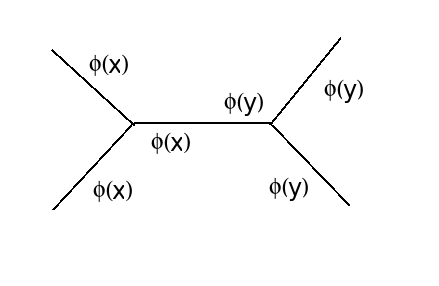
\includegraphics[width=2in]{feynman2.png}  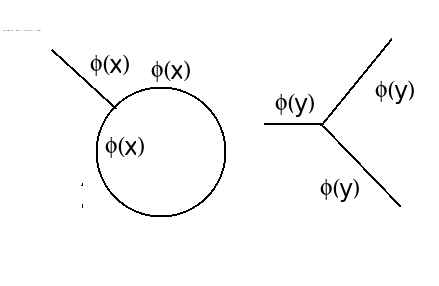
\includegraphics[width=2in]{feynman2_loop.png}


\skipline
包含$\contr{\hatphi(x)}{\hatphi(x)}$(右图)或者$\contr{\hatphi(y)}{\hatphi(y)}$的项里必然有一个粒子单独地未和其他粒子发生作用,所以描述的不是散射过程。关于这种圈图的物理诠释,我们以后再讲。


\ech
\end{frame}


\begin{frame}
\chtitle{要算的几个Feynman图}
\bch
所以我们要算的六个图为:
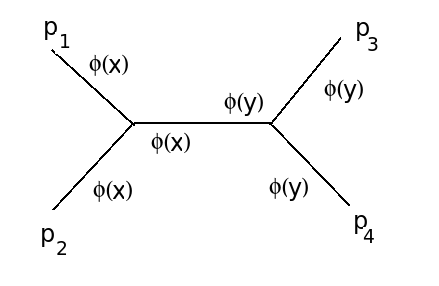
\includegraphics[width=1.5in]{feynman2_s_channel.png}  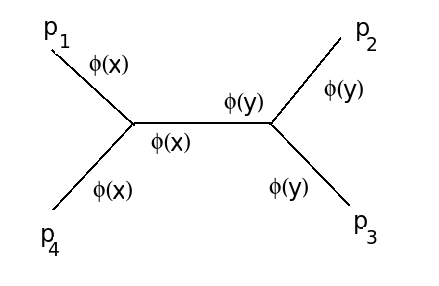
\includegraphics[width=1.5in]{feynman2_t_channel.png} 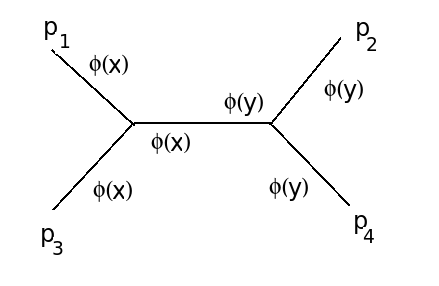
\includegraphics[width=1.5in]{feynman2_u_channel.png}

和三个把$x$,$y$互换的图

\ech
\end{frame}


\begin{frame}
\chtitle{s道Feynman图}
\bch

\bmini{0.5}
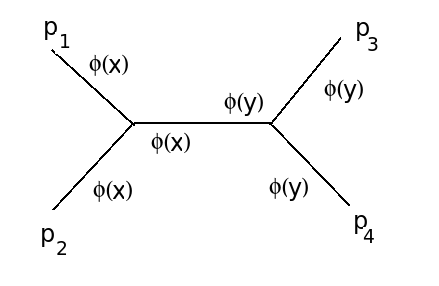
\includegraphics[width=1.5in]{feynman2_s_channel.png}
\emini
\bmini{0.4}
 + ($x$, $y$互换)
\emini
{\scriptsize
\bea
&& = (-\ii g)^2 \frac{(d^3\veck)^2}{4\sqrt{\omega_1\omega_2\omega_3\omega_4}}  \frac{1}{(2\pi)^6} \int d^4x\, \int d^4y\, e^{-\ii (p_1+p_2) x + (p_3+p_4)y} \contr{\hatphi{x}}{\hatphi(y)} \newl
&& = (-\ii g)^2 \frac{(d^3\veck)^2}{4\sqrt{\omega_1\omega_2\omega_3\omega_4}}  \frac{1}{(2\pi)^{10}} \int d^4x \int d^4y \int d^4 p\, e^{-\ii (p_1+p_2) x + (p_3+p_4)y} \frac{\ii e^{-ip(x-y)}}{p^2-m^2+i\epsilon} \newl
&& = (-\ii g)^2 \frac{(d^3\veck)^2}{4\sqrt{\omega_1\omega_2\omega_3\omega_4}}  \frac{1}{(2\pi)^2} \int d^4 p\, \delta(p_1+p_2+p)\delta(p_3+p_4+p) \frac{\ii}{p^2-m^2+i\epsilon} \newl
&& = (-\ii g)^2 \frac{1}{4\sqrt{\omega_1\omega_2\omega_3\omega_4}} \frac{\ii}{(p_1+p_2)^2-m^2}  \left(\frac{T}{V} \delta(p_1+p_2-p_3-p_4)d^4k\right) \newl
\eea
注:上面的计算中,把三个$\hatphi(x)$排序以及三个$\hatphi(y)$排序抵消了$\frac{1}{(3!)^2}$的因子,把$x$和$y$互换抵消了$\frac{1}{2}$因子。
}
\ech
\end{frame}



\begin{frame}
\chtitle{总结一下Feynman规则}
\bch
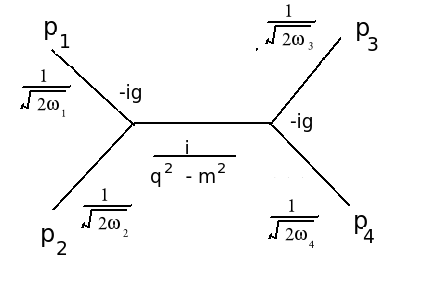
\includegraphics[width=2.5in]{feynman2_s_channel_diagram.png}
\begin{itemize}
\item{外线给出因子$\frac{1}{\sqrt{2\omega}}$}
\item{顶点给出因子$-ig$}
\item{内线给出因子$\frac{\ii}{q^2-m^2}$}
\end{itemize}
\ech
\end{frame}

\begin{frame}
\chtitle{利用Feynman规则来计算另两个图对散射振幅的贡献}
\bch
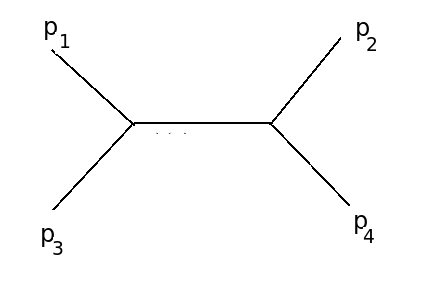
\includegraphics[width=2.2in]{feynman2_u_channel_simple.png} 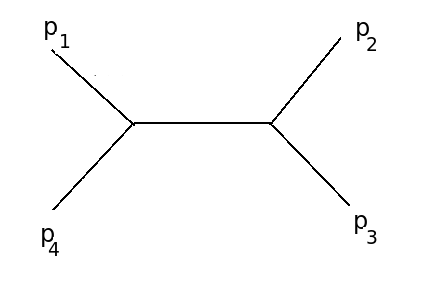
\includegraphics[width=2.2in]{feynman2_t_channel_simple.png} 

\ech
\end{frame}

\begin{frame}
\chtitle{最终答案}
\bch
{
\scriptsize
\bea
\calM &=& \frac{1}{4\sqrt{\omega_1\omega_2\omega_3\omega_4}} \newl
&& \times  \left[-\ii\lambda -  g^2\left(\frac{\ii}{(p_1+p_2)^2-m^2} + \frac{\ii}{(p_1-p_3)^2-m^2} + \frac{\ii}{(p_1-p_4)^2-m^2} \right)\right]
\eea
}
\ech
\end{frame}


\end{document}


